\subsubsection{Ανάπτυξη δυνάμεων στο ελαστικό}
Το ελαστικό αποτελεί το βασικό μηχανικό στοιχείο μέσω του οποίου το
όχημα αλληλεπιδρά με το οδόστρωμα. Μέσω της περιοχής επαφής
μεταφέρονται στο όχημα η κατακόρυφη δύναμη, η διαμήκης δύναμη και η
πλευρική δύναμη. Το πέλμα του ελαστικού (η επιφάνεια επαφής με το οδόστρομα) 
δεν είναι σταθερό, αλλά επηρεάζεται από το κατακόρυφο φορτίο, την πίεση, 
τη γωνία κάμπερ και τη γεωμετρία του ελαστικού \cite{Pacejka2012,Farroni2014TRT}.

\begin{figure}[htbp!]
    \centering
    \begin{tikzpicture}[
        >={Latex[length=2.2mm,width=1.6mm]},
        font=\small
      ]
      % ------------- Geometry -------------
      \def\R{4.0}
      \def\RE{3.7}
      \def\hCP{0.55}
      \def\tilt{0.18}
      \pgfmathsetmacro{\xC}{sqrt(\R*\R - (\RE-\hCP)*(\RE-\hCP))}
      \pgfmathsetmacro{\aR}{-asin((\RE-\hCP)/\R)}
      \pgfmathsetmacro{\aL}{180 - \aR}

      \coordinate (O) at (0,\RE);

      % ------------- Ground line + hatching (skip under the contact zone) -------------
      \draw[thick] (-\xC-3.8, 0) -- (\xC+3.8, 0);
      \pgfmathsetmacro{\xHg}{-\xC-\tilt}
      \pgfmathsetmacro{\xDg}{\xC}
      \foreach \x in {-5.2,-4.7,...,5.2} {
        \pgfmathparse{(\x < \xHg-0.15) || (\x > \xDg+0.15) ? int(1) : int(0)}
        \ifnum\pgfmathresult=1
          \draw[gray] (\x, 0) -- ++(-0.18,-0.28);
        \fi
      }

      % ------------- Tire outline: arc stops at top of bristles (y = hCP) -------------
      \draw[thick] ($ (O) + (\aR:\R) $)
            arc[start angle=\aR, end angle=\aL, radius=\R];
      \draw[thick] (-\xC, \hCP) -- (\xC, \hCP);

      % ------------- Bristles (brush model, braking: bottoms drag LEFT) -------------
      % Sticking region (right, x >= 0): tilt grows linearly from 0 at x=xC to \tilt at x=0
      % Sliding region  (left,  x < 0):  tilt fixed at \tilt (max deflection)
      \foreach \x in {0.0, 0.2, 0.4, ..., 2.6} {
        \pgfmathsetmacro{\loc}{\tilt * (1 - \x/\xC)}
        \draw[thin] (\x, \hCP) -- ++(-\loc, -\hCP);
      }
      \foreach \x in {-0.2, -0.4, -0.6, ..., -2.6} {
        \draw[thin] (\x, \hCP) -- ++(-\tilt, -\hCP);
      }

      % ------------- Named points -------------
      \coordinate (G) at (-\xC, \hCP);
      \coordinate (E) at (0, \hCP);
      \coordinate (C) at (\xC, \hCP);
      \coordinate (H) at (-\xC-\tilt, 0);
      \coordinate (F) at (-\tilt, 0);
      \coordinate (D) at (\xC, 0);
      \coordinate (A) at ($ (O) + (35:\R) $);
      \coordinate (B) at (\xC+1.1, 0);

      % Draw all point dots and non-conflicting labels here; F and B labels are
      % drawn LAST (after pressure arrows and hatching) so their white fill covers
      % whatever is underneath.
      \foreach \p in {G,E,C,H,F,D,A,B} \fill (\p) circle (1.6pt);
      \node[left=1pt of G]  {G};
      \node[above=-1pt of E]       {E};
      \node[below left=-1pt of H]  {H};
      \node[above right=-1pt of A] {A};

      \fill (O) circle (1.6pt);

      % ------------- Rotation Ω -------------
      \coordinate (Otop) at (0, \RE + \R + 0.35);
      \draw[thick, ->] ($ (Otop) + (170:0.55) $)
            arc[start angle=170, end angle=30, radius=0.55];
      \node[above=1.6cm of Otop, align=center]
        {Γωνιακή ταχύτητα περιστροφής\\ υπό πέδηση $\Omega$};

      % ------------- V_X -------------
      \draw[thick, ->] (O) -- ++(1.9, 0) node[below, midway] {$V_X$};

      % ------------- R -------------
      \draw[thick, ->] (O) -- (A) node[midway, above left=-3pt] {$R$};

      % ------------- R_E -------------
      \pgfmathsetmacro{\xLE}{-\R-0.4}
      \draw[thick, |<->|] (\xLE, 0) -- (\xLE, \RE) node[midway, left=1pt] {$R_E$};

      % ------------- V_X - Ω R_E > 0 -------------
      \node[anchor=west] at (\xC+1.4, 1.6) {$V_X - \Omega R_E > 0$};

      % ------------- Pressure distribution, aligned with ground contact H..D -------------
      \pgfmathsetmacro{\xHg}{-\xC-\tilt}
      \pgfmathsetmacro{\xDg}{\xC}
      \pgfmathsetmacro{\xMid}{(\xHg+\xDg)/2}
      \pgfmathsetmacro{\wHalf}{(\xDg-\xHg)/2}
      \foreach \k in {-5,-4,...,5} {
        \pgfmathsetmacro{\xp}{\xMid + \k*\wHalf/6}
        \pgfmathsetmacro{\hp}{0.92*(1 - (\k/6)*(\k/6))}
        \draw[->, gray!60!black, thick] (\xp, -0.05) -- (\xp, -0.05-\hp);
      }
   

      % ------------- Region brackets: separate at F on the ground -------------
      \def\yb{-2.7}
      \draw[decorate, decoration={brace, amplitude=5pt, mirror}] ($(F)+(0,\yb)$) -- ($(D)+(0,\yb)$);
      \node[anchor=north west] at ($(F)+(0.25,\yb-0.18)$) {Περιοχή προσκόλλησης};
      \draw[decorate, decoration={brace, amplitude=5pt, mirror}] ($(H)+(0,\yb-0.85)$) -- ($(F)+(0,\yb-0.85)$)
            node[midway, below=6pt] {Περιοχή ολίσθησης};

      \draw[dotted, gray] (H) -- ($(H)+(0,\yb-0.85)$);
      \draw[dotted, gray] (F) -- ($(F)+(0,\yb-0.85)$);
      \draw[dotted, gray] (D) -- ($(D)+(0,\yb)$);

      % ------------- F and B labels drawn LAST so white fill covers arrows / hatching
      \node[below=2pt of F,       fill=white, inner sep=3.5pt] {F};
      \node[below right=2pt of B, fill=white, inner sep=2.5pt] {B};
      \node[right=1pt of C, fill=white, inner sep=2.5pt] {C};
      \node[below right=-2pt of D, fill=white, inner sep=2.5pt] {D};
      \node[anchor=north,       fill=white, inner sep=2.5pt] at (\xMid, -1.15) {Κατανομή πίεσης};

    \end{tikzpicture}
    \caption{Παραμορφωμένο ελαστικό υπό πέδηση -- περιοχές προσκόλλησης \& ολίσθησης.}
    \label{fig:tire_contact}
\end{figure}


Η διαμήκης δύναμη $F_x$ σχετίζεται κυρίως με την πέδηση και την
επιτάχυνση. Αναπτύσσεται όταν υπάρχει διαφορά μεταξύ της περιφερειακής
ταχύτητας του ελαστικού και της ταχύτητας με την οποία μετακινείται το
κέντρο του τροχού. Η διαφορά αυτή περιγράφεται μέσω του συντελεστή
διαμήκους ολίσθησης $\kappa$. Συνέπεια αυτού του μηχανισμού είναι πως 
κατά την επιτάχυνση, η περιφερειακή
ταχύτητα του τροχού πρεπει να είναι μεγαλύτερη από την ταχύτητα του
οχήματος, ενώ κατά την πέδηση να είναι μικρότερη
\cite{Pacejka2012,Perantoni2014}.

Η πλευρική δύναμη $F_y$ αναπτύσσεται κατά την αλλαγή διεύθυνσης του
οχήματος. Η αντίστοιχη κινηματική ποσότητα είναι η γωνία ολίσθησης
$\alpha$, η οποία εκφράζει τη διαφορά μεταξύ της διεύθυνσης του επιπέδου
του τροχού και της διεύθυνσης της ταχύτητας στο σημείο επαφής. Μη
μηδενική γωνία ολίσθησης προκαλεί πλευρική παραμόρφωση του πέλματος και
συνεπώς ανάπτυξη πλευρικής δύναμης
\cite{Pacejka2012,Perantoni2014}.

\paragraph{Μοντέλο "βούρτσας" (brush model)}
Για την κατανόηση της παραγωγής των δυνάμεων χρησιμοποιείται συχνά κατ'αναλογία το
μοντέλο "βούρτσας" (\textit{brush model}). Στο μοντέλο αυτό, το πέλμα
θεωρείται ότι αποτελείται από μεγάλο αριθμό στοιχειωδών ελαστικών στοιχείων,
όπως οι ίνες μιας βούρτσας τα οποία συνδέουν τον σκελετό του ελαστικού 
με το οδόστρωμα. Τα στοιχεία αυτά μπορούν να
παραμορφώνονται τόσο στη διαμήκη όσο και στην πλευρική διεύθυνση μέσα
στην περιοχή επαφής \cite{Pacejka2012,Sakhnevych2022}.

Η επιφάνεια του πέλματος διακρίνεται στη βιβλιογραφία στην περιοχή προσκόλλησης (\textit{adhesion region})
και στην περιοχή ολίσθησης (\textit{sliding region}). Στην περιοχή προσκόλλησης, τα στοιχεία του πέλματος
παραμένουν σε επαφή χωρίς σχετική ολίσθηση με το οδόστρωμα. Η ελαστική
τους παραμόρφωση (σε συνδυασμό με τον ρυθμό παραμόρφωσης) δημιουργεί διατμητικές τάσεις,
οι οποίες παράγουν τις διαμήκεις ή τις πλευρικές δυνάμεις. Στην περιοχή
ολίσθησης, η παραμόρφωση των στοιχείων έχει φτάσει το διαθέσιμο όριο
τριβής και τα στοιχεία ολισθαίνουν ως προς το οδόστρωμα
\cite{Pacejka2012,Sakhnevych2022}.

Καθώς αυξάνεται η ολίσθηση, αυξάνεται αρχικά και η παραμόρφωση των
στοιχείων του πέλματος. Όταν η τοπική δύναμη που αναπτύσσεται σε ένα
στοιχείο υπερβεί το όριο τριβής, τότε αυτό ξεκινά να ολισθαίνει. 
Η μετάβαση αυτή δεν συμβαίνει ταυτόχρονα σε
ολόκληρο το πέλμα, αλλά αρχίζει τοπικά και
επεκτείνεται όσο αυξάνεται η ολίσθηση σχηματίζοντας δηλαδή τις περιοχές
ολίσθησης και προσκόλλησης \cite{Sakhnevych2022}.

Η συνολική διαμήκης και πλευρική δύναμη προκύπτει από το σύνολο των δυνάμεων
προσκόλλησης και ολίσθησης σε ολόκληρη την περιοχή επαφής. Για μικρές τιμές
ολίσθησης, η σχέση μεταξύ δύναμης και ολίσθησης είναι περίπου γραμμική
και χαρακτηρίζεται από τη διαμήκη ή την πλευρική ακαμψία του ελαστικού.
Σε μεγαλύτερες τιμές ολίσθησης, η σχέση γίνεται μη γραμμική και η δύναμη
τείνει σε μέγιστη τιμή, η οποία περιορίζεται από την τριβή μεταξύ
ελαστικού και οδοστρώματος \ref{fig:load_slip_curve_regions} \cite{Pacejka2012}.

\begin{figure}[ht!]
    \begin{center}
        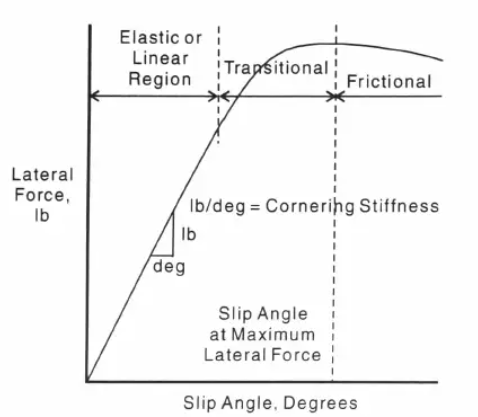
\includegraphics[width=0.6\textwidth]{figures/force-vs-slip_haney2004.png}
    \end{center}
    \caption{Περιοχές προσκόλλησης - ολίσθησης \cite{haney2025racing}}
    \label{fig:load_slip_curve_regions}
\end{figure}

Στην πραγματική λειτουργία, η διαμήκης και η πλευρική ολίσθηση
εμφανίζονται συχνά ταυτόχρονα. Η κατάσταση αυτή ονομάζεται συνδυασμένη
ολίσθηση. Για παράδειγμα, κατά την πέδηση μέσα σε στροφή, μέρος της
διαθέσιμης πρόσφυσης χρησιμοποιείται για την παραγωγή διαμήκους δύναμης
και το υπόλοιπο για την παραγωγή πλευρικής δύναμης. Για τον λόγο αυτό,
η μέγιστη πλευρική ή διαμήκης δύναμη μειώνεται όταν το ελαστικό
λειτουργεί ταυτόχρονα σε πέδηση ή επιτάχυνση και σε πλευρική ολίσθηση
\cite{Pacejka2012,Perantoni2014}. Στο ιδεατό ανάλογο μοντέλο brush, αυτό
θα ήταν άμεσα προφανές αν θεωρήσει κανείς τις ίνες της βούρτσας ως ισοτροπικές.
Σε αυτή την περίπτωση, σε κάθε διεύθυνση καθεμία ίνα έχει την ίδια διαθέσιμη
πρόσφυση, οπότε αγνοώντας τη γεωμετρία του ελαστικού, σε ενα επίπεδο διαμήκους και
πλευρικής δύναμης, η διαθέσιμη πρόσφυση του ελαστικού θα περιγραφόταν με έναν τέλειο κύκλο.
Ένα τέτοιο διάγραμμα ονομάζεται traction envelope. Στην πραγματικότητα 
τα ελαστικά λόγω της κατασκευής τους αλλά και της γεωμετρίας τους,
παρουσιάζουν ανισότροπη συμπεριφορά, και το traction envelope συνήθως
έχει τη μορφή έλλειψης, γι αυτό και καλείται συχνά traction ellipse. 

\paragraph{Φαινόμενο load sensitivity.}
Ο συντελεστής τριβής $\mu$ δεν είναι σταθερός αλλά μειώνεται ελαφρά καθώς αυξάνεται το
κατακόρυφο φορτίο.

Η φυσική βάση αυτού του φαινομένου έγκειται στη μη-γραμμική ελαστικότητα του ελαστομερούς
υπό πίεση: σε μεγάλα φορτία ο μηχανισμός προσκόλλησης φτάνει σε κορεσμό. Πρακτικά, αυτό σημαίνει
ότι κατά τη μεταφορά φορτίου σε μια στροφή ο επιφορτισμένος τροχός κερδίζει λιγότερη πρόσφυση
από ό,τι χάνει ο αποφορτισμένος. Αυτός ο μηχανισμός είναι και στο μεγαλύτερο βαθμό ο λόγος για τον
οποίο επιθυμείται χαμηλό κέντρο βάρους σε αγωνιστικές εφαρμογές (σχέσεις \ref{eq:Fz_long}, \ref{eq:Fz_lat})
-- ελαχιστοποιώντας το ύψος του κέντρου βάρους ελαχιστοποιούμε και το ποσό πρόσφυσης που "χάνεται".


\paragraph{Μαθηματικά μοντέλα ελαστικών}
Είναι προφανές λοιπόν πως τα ελαστικά αποτελούν ίσως τον σημαντικότερο
παράγοντα στις επιδόσεις ενός οχήματος και η ακριβής μοντελοποίησή τους
χρήζει ιδιαίτερου ενδιαφέροντος. Στην πράξη, λόγω και της έντονης πολυπλοκότητας
στους μηχανισμούς ανάπτυξης φορτίων, χρησιμοποιούνται ημιεμπειρικά παραμετρικά 
μαθηματικά μοντέλα τέτοιας μορφής όπως στις (\cref{eq:longitudinal_tyre_force, eq:lateral_tyre_force}) τα οποία σχεδιάζονται έτσι ώστε να μπορούν να αποτυπώσουν
τη συμπεριφορά των ελαστικών όσο το δυνατό ακριβέστερα προσαρμόζοντάς τα σε 
πειραματικά δεδομένα . Ίσως το πιο διαδεδομένο ημιεμπειρικό μοντέλο πλέον είναι
η Magic Formula του Pacejka \cite{Pacejka2012,Sakhnevych2022}.

\begin{equation}
F_x = F_x\left(F_z,\kappa,\alpha\right),
\label{eq:longitudinal_tyre_force}
\end{equation}

\begin{equation}
F_y = F_y\left(F_z,\kappa,\alpha\right).
\label{eq:lateral_tyre_force}
\end{equation}

